% !TeX root = main.tex
% !TeX spellcheck = de_DE
% !TeX encoding = utf8

\chapter{Channel Models}
As the encoded message is passed through a channel I will introduce some basic channel models in this chapter. I will only work with binary codes throughout this thesis. For binary codes it is convenient to use $\{ +1, -1\}$
 as the alphabet. This simplifies the calculations of LLRs likewise it makes the bit energy $E_b$ simple. Also the channel is memoryless, this may sound confusing at first when dealing with storage devices, but it says that each symbol is independently \todo{better word}mangled by the channel. The input to the channel is in the input alphabet $\mathcal{X} = \{1, -1\}$. Whereas the the output alphabet $\mathcal{Y}$ will change depending on the channel. Now when transmitting a codeword $c \in \mathcal{X}^n$ the channel outputs $y \in \mathcal{Y}^n$ and it is the receivers task to compute the original codeword $c$ from $y$. Ideally this is done with few errors and close to the channel capacity.

\section{Binary Erasure Channel (BEC)}
The binary erasure channel is characterized with a single parameter $0 \leq \alpha < 1$ the erasure probability. The symbol for an erasure is $?$, therefore the output alphabet is $\mathcal{Y} = \{1, -1, ?\}$. The channel outputs $x$ with probability $1 - \alpha$ and $?$ with probability $\alpha$. \cref{bec_schema} shows the transitions for a BEC. So for a codeword with large length $n$ there will be $(1 - \alpha)n$ correct symbols, this suggests that the maximum rate is $1 - \alpha$. Elias\cite{El55} shows that this rate can be archived and also proves that this is the capacity.

\begin{figure}
	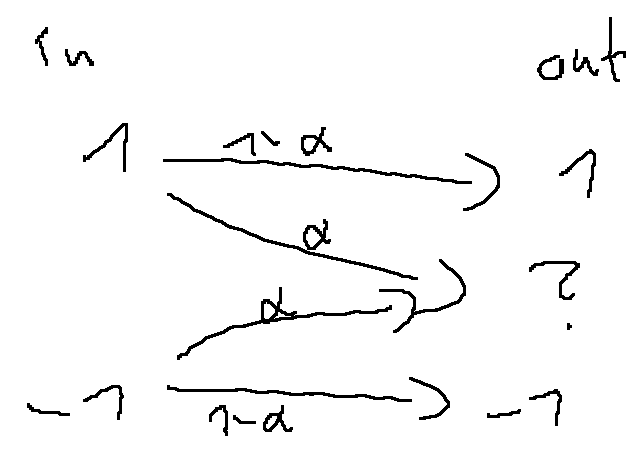
\includegraphics[width=5cm]{bec_schema.png}
	\centering
	\caption{Symmetric binary erasure channel}
	\label{bec_schema}
\end{figure}


\section{BSC}
A binary symmetric channel has the output alphabet $\mathcal{Y} = \{1, -1\}$. An incoming symbol has the probability $p$ to create a crossover. With probability $1 - p$ the symbol is correctly transmitted and with probability $p$ it is flipped. In \cref{bsc_schema} a graph shows these probabilities. A binary symmetric channel with crossover probability $p$ has the capacity $1 - H(p)$ with $H(p) = -p \log_2 p - (1 - p) \log_2 (1 - p)$ being the binary entropy function.

\begin{figure}
	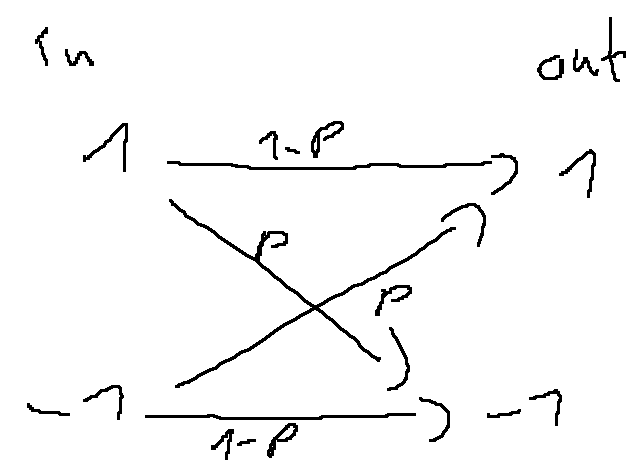
\includegraphics[width=5cm]{bsc_schema.png}
	\centering
	\caption{Symmetric binary symmetric channel}
	\label{bsc_schema}
\end{figure}

\section{Additive White Gaussian Noise Channel}
The additive white gaussian noise (AWGN) channel is the most important noise model for me as it characterizes flash memory well. It has a continuos output alphabet $\mathcal{Y}$. The model for the channel is $y = x + z$ where the input is $x \in \mathcal{X}$. $z$ is a variable with normal distribution with $0$ mean and variance $\sigma^2$. It has the distribution $f(z) = \frac{1}{\sqrt{2 \pi \sigma^2}}\exp(-\frac{z^2}{2 \sigma^2})$. The capacity for this channel is $\frac{1}{2} \log_2(1 + \frac{1}{\sigma^2})$ as the Shannon limit shows. Often it is preferable to allow scaling of the input, so we use a signal to noise ratio $E_b / \sigma^2$. This allows the inputs to be arbitrary values then $E_b$ is the energy of the transmission of a single bit. The $\sigma^2$ is frequently called $N_0$, the energy of the noise that is added in a single bit transmission. When using $E_b / N_0$ the capacity is $\frac{1}{2} \log_2(1 + \frac{E_b}{N_0})$. For example when having a rate of $\frac{1}{2}$ we get a minimum signal to noise ratio required of 1.

\begin{figure}
	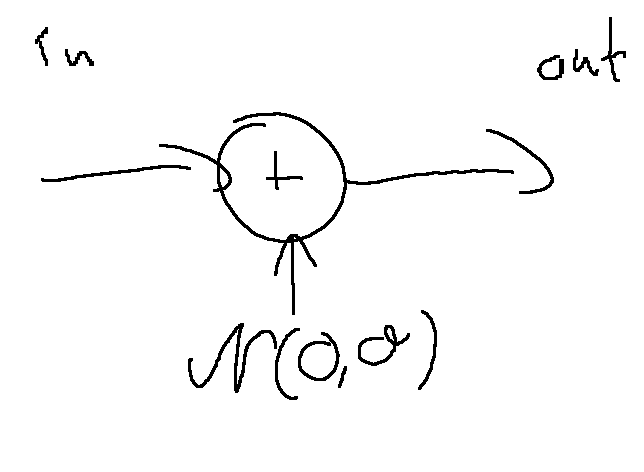
\includegraphics[width=5cm]{awgn_schema.png}
	\centering
	\caption{Additive White Gaussian Noise Channel}
	\label{awgn_schema}
\end{figure}
